\documentclass{report}

%common packages
\usepackage{float}
\usepackage{graphicx}
\usepackage{amsmath}
\usepackage{mathtools}

\begin{document}
	
		
	\begin{figure}[H]  % [H] - stay here
		\centering      %pictures too big will cause errors
		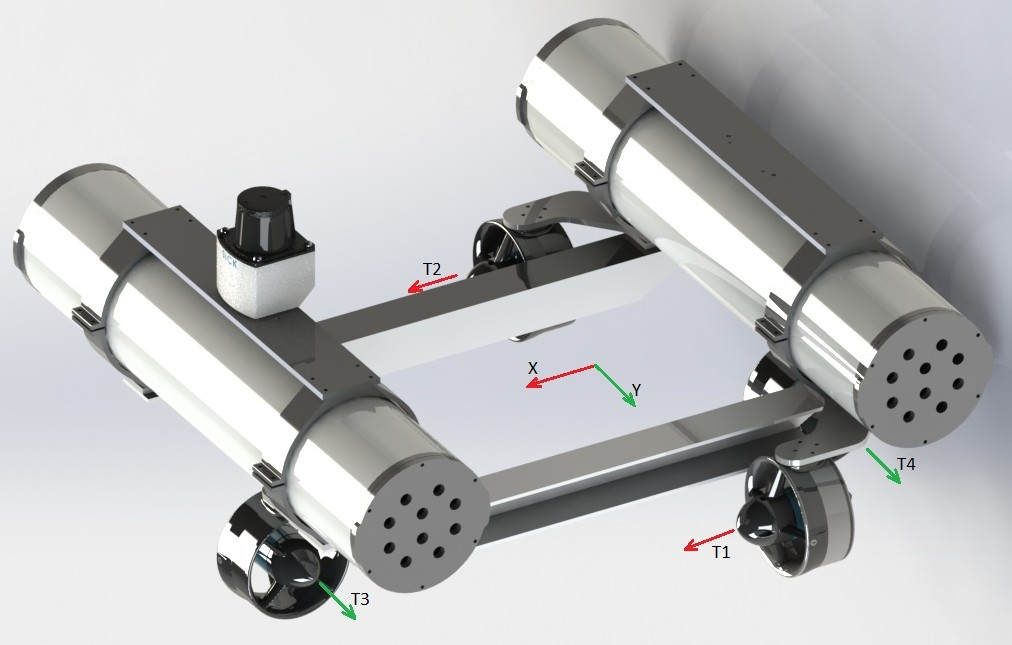
\includegraphics[height=8cm]{figures/Mallard_skewed}
		\caption{Mallard and its thruster configuration. Arrows show forward force direction produced by each thruster $(T_1,T_2,T_3$ and $T_4 )$.}	
		\label{mallard_skewed}
	\end{figure}

	
		
		
	\begin{figure}[H]  % [H] - stay here
		\centering      %pictures too big will cause errors
		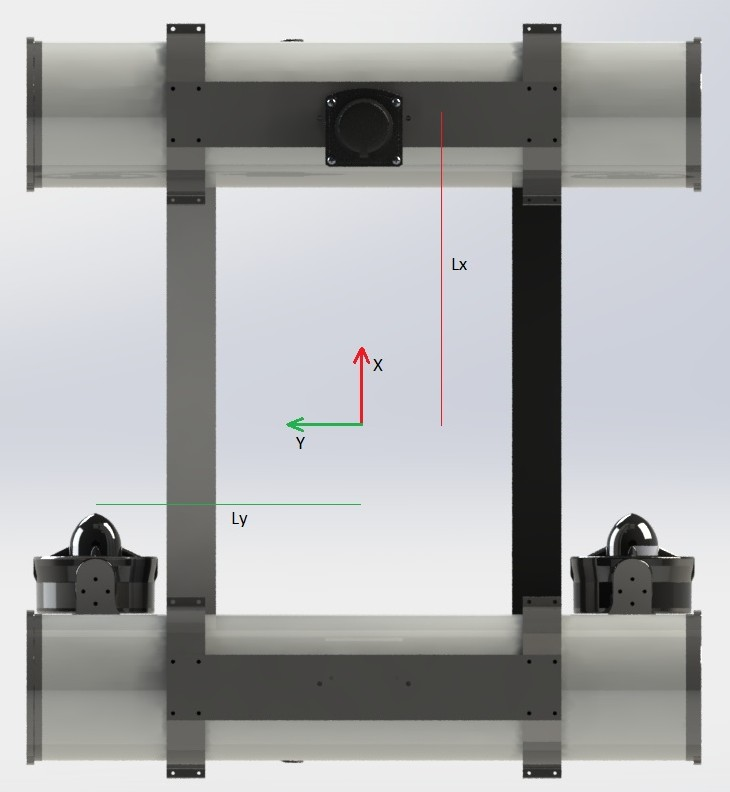
\includegraphics[height=9cm]{figures/Mallard_top}
		\caption{Top view. Moment arms $L_x$ and $L_y$ that are measured 
			from the centre of Mallard, i.e. half the distance between thrusters. }	
		\label{mallard_top}
	\end{figure}
	
	\noindent
	$\boldsymbol{\tau} = [U~V~R]^T$ - velocity vector in body (Mallard's) reference frame \\
	$\boldsymbol{u} =  [T_1~T_2~T_3~T_4]^T$ - forces to be allocated for each thruster\\
	$L_x,L_y$ - moment arms\\\\
	
	
	\begin{equation}
	\begin{aligned}
		\begin{bmatrix}
		U \\
		V \\
		R \\
		\end{bmatrix}
		=
		\begin{bmatrix}
		1   & 1 & 0 & 0\\
		0   & 0 & 1 & 1\\
		L_y & -L_y & L_x & -L_x
		\end{bmatrix}
		\begin{bmatrix}
		T_1 \\
		T_2 \\
		T_3 \\
		T_4 \\
		\end{bmatrix}
	\end{aligned}
	\end{equation}
	

	
	\begin{equation}
	\begin{aligned}
		\boldsymbol{\tau} = \boldsymbol{B} * \boldsymbol{u}
	\end{aligned}
	\end{equation}
	
	\begin{equation}
	\begin{aligned}
		\boldsymbol{u} = \boldsymbol{B^{+}} * \boldsymbol{\tau}
	\end{aligned}
	\end{equation}
	
	\begin{equation}
	\begin{aligned}
	\begin{bmatrix}
		T_1 \\
		T_2 \\
		T_3 \\
		T_4 \\
	\end{bmatrix}
	=
	\begin{bmatrix*}[r]
	0.5 &  0  &  a\\
	0.5 &  0  & -a\\
	0   & 0.5 &  b\\
	0   & 0.5 & -b
	\end{bmatrix*}
	\begin{bmatrix}
		U \\
		V \\
		R \\
	\end{bmatrix}
	\end{aligned}
	\end{equation}
	
	

	
	
	
	
		
	
	
	
		
\end{document}